%=================ESTADO DEL ARTE Y MARCO TEÓRICO=================

%=================ESTADO DEL ARTE=================
\section{Estado del arte}
%\TODO \textbf{Recuerdo que había que diferenciar entre los artículos y las tesis pero no sé cómo hacerlo. ¿Así está bien?} 
\subsection{Tesis}
	Diana Olvera y José Gonzáles proponen un Sistema de Monitoreo de Signos Vitales capaz de monitorear la presión arterial, el ritmo cardíaco y la temperatura corporal desde el mismo dispositivo con la finalidad de que estas mediciones puedan ser realizadas desde cualquier lugar  sin tener un amplio conocimiento en medicina para su uso. Este sistema se desarrolló implementando el PIC18F4550 para procesar las señales provenientes de los sensores y desplegarlos en un display LCD[2].\\
	
	En el “Sistema de monitoreo remoto y evaluación de signos vitales en pacientes con enfermedades crónicas”, López, Guerrero y Ramos proponen un sistema que sensa los signos vitales de un paciente y utiliza bluetooth y WiFi para transmitir dicha información a un dispositivo móvil encargado de evaluarla y alertar a alguna persona en caso de requerirse[3].\\
	
	Existe un prototipo de hardware/software propuesto por Chávez, Martínez y Torres el cual mediante el uso de un sistema embebido dentro de un microcontrolador DSPIC30F3013 ayuda en el procesamiento, medición y envío mediante una red, tres signos vitales (presión arterial, frecuencia cardiaca y temperatura corporal), dichas mediciones son procesadas por el microcontrolador y enviadas mediante UART hacia un controlador Ethernet para ser recibidas y mostradas por una aplicación diseñada para el usuario[4]. \\

\subsection{Artículos}
	El prototipo diseñado por Li, Cummings, Lan, Graves y Wu en [5], es un sistema de monitoreo de la frecuencia cardiaca y respiratoria de bebés. Está compuesto por una unidad de monitoreo y una unidad receptora. Con un circuito de radiofrecuencia es capaz de producir y recibir señales de radio para la detección de los signos vitales sin la necesidad de que un sensor tenga contacto con el bebé. Utiliza un microcontrolador para procesar la señal recibida y un chip de comunicación XBee para la comunicación inalámbrica con el módulo receptor. \\
	
	En el artículo [6], Girbau, Ramos , Lázaro y Villarino, propone un sistema para el monitoreo de los signos vitales utilizando un radar Doppler y la interfaz Zigbee para enviar la información del sensor de microondas. En este sistema se detecta la respiración y la frecuencia cardiaca, se adquiere con el sistema Zigbee y se transmite vía radiofrecuencia. Permite el monitoreo simultáneo de varias personas localizadas en diferentes nodos Zigbee. \\
	
	Cruz y Barros proponen en [7] el uso de PDAs la adquisición de los signos vitales y su transmisión a un servidor de cuidados de la salud en donde un especialista pueda analizar el electrocardiograma (ECG) generado. Para la adquisición del ECG utiliza electrodos en el paciente. Y para la sincronización de los datos almacenados en la PDA con el servidor, requiere de una conexión a Internet.
	
%=================MARCO TEÓRICO=================
\section{Marco teórico}
	\subsection{Internet de las cosas (IoT)}
	El Internet de las cosas (IoT) es un concepto y un paradigma que considera la presencia generalizada en el entorno de una variedad de cosas/objetos que contienen tecnología integrada para comunicarse a través de conexiones alámbricas e inalámbricas con el fin de interactuar entre sí y cooperar con otras cosas/objetos para crear nuevas aplicaciones/servicios y alcanzar objetivos comunes.
	
	\subsection{Sistemas embebidos}
	Los sistemas embebidos son combinaciones de software y hardware con restricciones de recursos que se dedica a una aplicación o parte específica de una aplicación o sistema más grande. Son controlados por una computadora incrustada en ellos, lo que implica que se encuentra dentro del sistema general, oculto a la vista, formando una parte integral de un conjunto mayor. Es probable que dicha computadora sea un microprocesador o microcontrolador.\\
	
	Los sistemas embebidos tienen varias características comunes:
	\begin{itemize}
		\item Un sistema embebido generalmente ejecuta solo un programa, repetidamente.
		\item Su diseño debe ser optimizado para reducir costo y espacio. Contienen sólo los recursos de hardware suficientes para cumplir con  los  requerimientos  de  funcionalidad  de  la  aplicación.
		\item Muchos sistemas embebidos deben reaccionar continuamente a los cambios en el entorno del sistema y deben calcular ciertos resultados sin demora.
	\end{itemize}
	\subsubsection{Arquitectura de los sistemas embebidos}
	\TOCHK{Agregar imagen y descripción de su arquitectura}
	\subsection{Signos vitales}
	Los signos vitales son indicadores que reflejan el estado fisiológico de los órganos vitales (cerebro, corazón, pulmones). Sus variaciones expresan cambios que ocurren en el organismo, algunos de índole fisiológico y otros de tipo patológico. Los valores considerados normales se ubican dentro de rangos y estos rangos varían según la edad y en algunos casos también con el sexo. Los cuatros principales signos vitales son: 
	\begin{enumerate}
		\item Frecuencia cardíaca.
		\item Frecuencia respiratoria.
		\item Presión arterial.
		\item Temperatura.
	\end{enumerate}

	\subsubsection{Frecuencia cardíaca}
	El pulso está representado por la expansión rítmica de las arterias producida por el pasaje de sangre que es bombeada por el corazón originada en la contracción del ventrículo izquierdo, y que resulta en la expansión y contracción regular del calibre de las arterias; representa el rendimiento del latido cardíaco y la adaptación de las arterias.\\
	
	Los valores del Pulso arterial se miden a partir de la “Frecuencia Cardíaca” o sea el número de pulsaciones o latidos que ocurren en “Un Minuto”. La frecuencia cardíaca varía dependiendo de diferentes factores, como: la edad, sexo, actividad física, estado emocional, fiebre, medicamentos y hemorragias.
	
	\begin{table}[htbp]
		\begin{center}
			\begin{tabular}{|l|l|}
				\hline
				\textbf{Edad} & \textbf{Pulsaciones por minuto} \\
				\hline \hline
				Recién nacido & 120 - 170  \\
				\hline
				Lactante menor & 120 - 160  \\
				\hline
				Lactante mayor & 110 - 130  \\
				\hline
				De 2 a 4 años & 100 - 120  \\
				\hline
				De 6 a 8 años & 100 - 115  \\
				\hline
				Adulto & 60 - 80  \\
				\hline
			\end{tabular}
			\caption{Valores normales de frecuencia cardíaca.}
		\end{center}
	\end{table}

	\subsubsection{Frecuencia respiratoria}
	Respiración es el término que se utiliza para indicar el intercambio de oxígeno y dióxido de carbono que se lleva a cabo en los pulmones y tejidos. El ciclo respiratorio comprende una fase de inspiración y otra de espiración:
	\begin{itemize}
		\item \textbf{Inspiración:} fase activa; se inicia con la contracción del diafragma y los músculos intercostales.
		\item \textbf{Espiración:} fase pasiva; depende de la elasticidad pulmonar.
	\end{itemize}
	
	La frecuencia respiratoria es el número de respiraciones que suceden en un minuto, y comprende el proceso de inhalación y exhalación.\\
	
	La frecuencia se mide por lo general cuando una persona está en reposo y consiste simplemente en contar la cantidad de respiraciones durante un minuto cada vez que se eleva el pecho. La frecuencia respiratoria puede aumentar con la fiebre, las enfermedades y otras afecciones médicas.
	
	\begin{table}[htbp]
		\begin{center}
			\begin{tabular}{|l|l|}
				\hline
				\textbf{Edad} & \textbf{Respiraciones por minuto} \\
				\hline \hline
				Recién nacido & 30 - 80  \\
				\hline
				Lactante menor & 20 - 40  \\
				\hline
				Lactante mayor & 20- 30  \\
				\hline
				De 2 a 4 años & 20- 30  \\
				\hline
				De 6 a 8 años & 20 - 25  \\
				\hline
				Adulto & 12 -20  \\
				\hline
			\end{tabular}
			\caption{Valores normales de frecuencia respiratoria.}
		\end{center}
	\end{table}
	
	\subsubsection{Presión arterial}
	Es una medida de la presión que ejerce la sangre sobre las paredes arteriales en su impulso a través de las arterias. Debido a que la sangre se mueve en forma de ondas, existen dos tipos de medidas de presión: la presión sistólica, que es la presión de la sangre debida a la contracción de los ventrículos, es decir, la presión máxima; y la presión diastólica, que es la presión que queda cuando los ventrículos se relajan; ésta es la presión mínima. Tanto la presión sistólica como la diastólica se registran en "mm de Hg" (milímetros de mercurio). \\
	
	La Presión arterial media se calcula con la siguiente fórmula: 
	
	\begin{center}
		\textit{PA = Presión sistólica – Presión diastólica / 3 + Presión diastólica.}
	\end{center}
	
	\begin{table}[htbp]
		\begin{center}
			\begin{tabular}{|l|l|l|}
				\hline
				\textbf{Edad} & \textbf{Presión Sistólica (mmHg)} & \textbf{Presión Diastólica (mmHg)} \\
				\hline \hline
				Lactante menor & 60 - 90 & 30 - 60 \\
				\hline
				2 años  & 78 - 112 & 48 - 78 \\
				\hline
				4 años & 85 - 114 & 52 - 85 \\
				\hline
				8 años & 95 - 135 & 58 - 88 \\
				\hline
				Adulto & 100 - 140 & 60 - 90 \\
				\hline
			\end{tabular}
			\caption{Valores normales de la presión arterial.}
		\end{center}
	\end{table}
	
	\subsubsection{Temperatura}
	La temperatura corporal representa el estado térmico del organismo y expresa el balance entre la producción de calor en el cuerpo (termogénesis) y la pérdida (termólisis). En el hombre, un conjunto de funciones fisiológicas contribuye a mantener constante la temperatura, que se mide por medio de termómetros. La temperatura normal del cuerpo varía según el sexo, la actividad reciente, el consumo de alimentos y líquidos, la hora del día y, en las mujeres, la etapa del ciclo menstrual. 
	
	\begin{table}[htbp]
		\begin{center}
			\begin{tabular}{|l|l|}
				\hline
				\textbf{Edad} & \textbf{Grados Celsius} \\
				\hline \hline
				Recién nacido & 36.1 - 37.7  \\
				\hline
				Lactante & 37.2  \\
				\hline
				De 2 a 8 años & 37.0  \\
				\hline
				Adulto & 36.0 - 37.0  \\
				\hline
			\end{tabular}
			\caption{Valores normales de temperatura.}
		\end{center}
	\end{table}
	
	\subsection{Sensores de temperatura}
	Un sensor de temperatura es un dispositivo que proporciona la medición de temperatura a través de una señal eléctrica. \\
		
	Se utilizan en diversas aplicaciones tales como elaboración de alimentos, climatización para control ambiental, dispositivos médicos, manipulación de productos químicos y control de dispositivos en el sector automotriz, entre otros. \\
		
	Los sensores de temperatura se utilizan para asegurar que la temperatura de algún objeto se encuentre dentro de un cierto rango, lo que proporciona seguridad en el uso de la aplicación. \\
		
	Dependiendo del dispositivo en el que se instalará el sensor de temperatura y el propósito de la aplicación, se deberá utilizar un tipo específico de sensor para medir la temperatura de manera precisa y eficiente, pues en muchos casos la capacidad de respuesta y precisión del circuito de detección puede ser crítica para una pronta decisión.\\
	
	Algunos de los tipos más comunes de sensores de temperatura son los siguientes:
	
		\begin{itemize}
			\item \textbf{Termistores:} Un termistor es un elemento con una resistencia eléctrica que cambia en respuesta a la temperatura. Este nombre se deriva del término más descriptivo "resistencia térmicamente sensible".\\
						
			Los termistores son un tipo de semiconductor, lo que significa que tienen mayor resistencia que los materiales conductores, pero menor resistencia que los materiales aislantes. La relación entre la temperatura de un termistor y su resistencia depende en gran medida de los materiales de los que está compuesta.\\
			
			Existen dos clases de termistores los que presentan un coeficiente negativo de temperatura (NTC), cuya resistencia disminuye con la temperatura y coeficiente positivo con la temperatura  (PTC) cuya resistencia aumenta con la temperatura. Los termistores NTC son los más usados para medición de temperatura.
			
			\item \textbf{Circuitos integrados:}
			\item \textbf{Termopares:} Los termopares se usan comúnmente para medir temperaturas más altas y rangos de temperatura más grandes.\\
			
			Este tipo de sensor de temperatura consta de dos cables de diferentes metales conectados en dos puntos. La tensión variable entre estos dos puntos refleja cambios proporcionales en la temperatura. La precisión es baja, de 0.5 $^{\circ}$C a 5 $^{\circ}$C. Sin embargo, operan en el rango de temperatura más amplio, de -200 $^{\circ}$C a 1750 $^{\circ}$C.			
		\end{itemize}
	
	\subsection{Sensores de pulso}
		\begin{itemize}
			\item Fotopletismógrafos
			\item ECG
		\end{itemize}
	
	\subsection{Redes inalámbricas}	
	Las redes inalámbricas son conjuntos de dispositivos informáticos comunicados entre sí  sin la necesidad de utilizar cables de ningún tipo. Las redes inalámbricas funcionan de manera similar a las redes cableadas, sin embargo, las redes inalámbricas deben convertir las señales de información en una forma adecuada para la transmisión a través del medio de aire. \\
	
	Las redes inalámbricas se pueden clasificar en cuatro grupos específicos según el área de aplicación y el alcance de la señal, como se muestra en la figura . Se llama alcance a la distancia máxima a la que pueden situarse las dos partes de la comunicación inalámbrica.
	
	\begin{figure}[htbp!]
		\centering
		\fbox{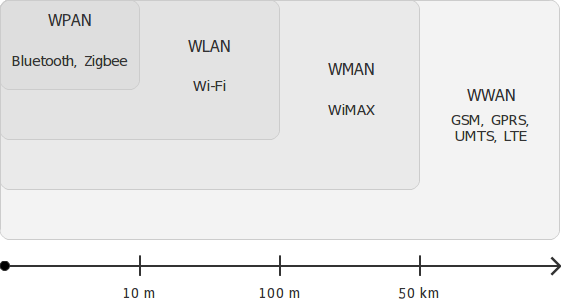
\includegraphics[width=0.8\textwidth]{images/marcoTeorico/redesInalambricas.png}}
		\caption{Arquitectura del sistema.}
		\label{fig:tiposRedes}
	\end{figure}
	
	
	\subsubsection{\textbf{Redes inalámbricas de área personal (Wireless Personal-Area Networks - WPAN)}}
	Las redes inalámbricas de área personal permiten la comunicación en un rango de distancias muy corto, unos 10 metros, baja velocidad, menos de 1 Mbps y con necesidad de visión sin obstáculos.\\
	
	Una conexión realizada a través de una WPAN implica poca o ninguna infraestructura o conectividad directa fuera del enlace establecido. Esto permite soluciones pequeñas, eficientes en energía y de bajo coste que pueden ser implementadas en una amplia gama de dispositivos informáticos y de comunicación portátil y móvil, como ordenadores, PDA, impresoras, ratones, micrófonos, auriculares, etc.
	
	\subsubsection{\textbf{Redes inalámbricas de área local (Wireless Local-Area Networks - WLAN)}}
	Las redes inalámbricas de área local (WLAN) están diseñadas para proporcionar acceso inalámbrico en zonas con un rango típico de hasta 100 metros y son utilizadas dentro de un mismo edificio o grupo de edificios. Esto proporciona a los usuarios la capacidad de moverse dentro de un área de cobertura local y permanecer conectado a la red. 
	
	\subsubsection{\textbf{Redes inalámbricas de área metropolitana (Wireless Metropolitan-Area Networks - WMAN)}}
	Las redes inalámbricas de área metropolitana (WMAN) forman el tercer grupo de redes inalámbricas. Se llama redes inalámbricas de área metropolitana, WMAN (Wireless Metropolitan Area Networks), a aquellas redes que tienen una cobertura desde unos cientos de metros hasta varios kilómetros. El objetivo es poder cubrir el área de una ciudad o entorno metropolitano. 
	
	\subsubsection{\textbf{inalámbricas de área amplia (Wireless Wide-Area Networks - WWAN)}}
	Las redes inalámbricas de área amplia se extienden a miles de kilómetros y suelen utilizar frecuencias con licencia. Este tipo de redes se pueden mantener en grandes áreas, tales como ciudades o países, a través de los múltiples sistemas de satélites o ubicaciones con antena atendidos por un proveedor de servicios de Internet. Las WWAN permiten la interconexión de varios sistemas de comunicaciones ayudando a que ésta sea cada vez más globalizada.

	\subsection{Tecnologías inalámbricas}
	Existen muchas tecnologías diferentes que difieren en la frecuencia de transmisión utilizada, la velocidad y el alcance de sus transmisiones. Cada una de esas tecnologías posee diferentes características que la hacen adecuada para diferentes tipos de aplicaciones. Asimismo existen diferentes tecnologías que pueden ser implementadas al mismo tipo de aplicación. Algunas de las tecnologías más significativas y con mayor penetración en el mercado son las siguientes:
	
	\subsubsection{Bluetooth}
	Bluetooth es un enlace radio de corto alcance que aparece asociado a las Redes de Área Personal Inalámbricas (WPAN) y pertenece al estándar IEEE 802.15.1. Originalmente Bluetooth fue diseñado para comunicaciones omnidireccionales (punto a multipunto), de bajo consumo de energía, corto alcance y con dispositivos baratos, reemplazando el uso de cables y conectando los dispositivos a través de una conexión ad hoc por radio. \\
		
	Bluetooth trabaja en el rango de frecuencias de 2,402 GHz a 2,480 GHz (Banda ISM). Los terminales pueden estar en movimiento y no tener línea de vista entre sí; además, las velocidades de transmisión oscilan entre 720kbps y 1 Mbps. 
	
	\subsubsection{Zigbee}
	ZigBee está basado en el estándar IEEE 802.15.4 que fue desarrollado como un estándar global abierto para abordar las necesidades de fácil aplicación, alta fiabilidad, bajo costo, bajo consumo y bajas velocidades de transmisión de datos en redes de dispositivos inalámbricos.\\
		
	Zigbee fue creado con  con la finalidad de promover el desarrollo e implantación de una tecnología inalámbrica bidireccional de bajo coste vía radio, para usarla en dispositivos de domótica, automatización de edificios (inmótica), control industrial, periféricos de PC o sensores médicos.  Tiene velocidades comprendidas entre 20Kbps y 250Kbps y rangos de 10 m a 75 m y opera en las bandas sin licencia 2.4 GHz, 900 MHz y 868 MHz, lo suficiente para satisfacer las necesidades de un sensor y de automatización usando redes inalámbricas.
	
	\subsubsection{Familia IEEE 802.11 (WI-FI)}
	
	
	\subsubsection{WiMAX}
	
	
	\subsubsection{GSM (Global System for Mobile Comunications)}
	GSM (Sistema Global para Comunicaciones Móviles) es una tecnología celular digital abierta que se utiliza para transmitir servicios móviles de voz y datos. GSM admite llamadas de voz y velocidades de transferencia de datos de hasta 9.6 kbps, junto con la transmisión de SMS (Servicio de Mensajes Cortos). \\

GSM opera en bandas y espectros armonizados en la mayor parte del mundo, combinado con la capacidad de roaming internacional de GSM, permite a los viajeros acceder a los mismos servicios móviles en el hogar y en el extranjero. GSM permite llegar a individuos a través del mismo número de móvil en hasta 219 países. \\

Las redes terrestres GSM ahora cubren más del 90\% de la población mundial. El servicio de roaming por satélite GSM también ha ampliado el acceso a servicios en áreas donde la cobertura terrestre no está disponible.

	